\documentclass[12pt,a4paper]{article}
\usepackage[utf8]{inputenc}
\usepackage{amsmath}
\usepackage{amsfonts}
\usepackage{amssymb}
\usepackage{float}
\usepackage{csvsimple}
\usepackage{enumerate}
\usepackage{hyperref}
\usepackage{graphicx}
\usepackage{gensymb}
\usepackage{txfonts}
\usepackage{listings}
\usepackage{cleveref}
\usepackage{xcolor}
\parindent 0px
\usepackage[none]{hyphenat}
\usepackage{listings} %Package for the enviroment in which we write code 
\usepackage[left=1cm,right=1cm,top=2cm]{geometry}
\pagenumbering{arabic}
%Some custom colours
\definecolor{codegreen}{rgb}{0,0.6,0}
\definecolor{codegray}{rgb}{0.5,0.5,0.5}
\definecolor{codepurple}{rgb}{0.58,0,0.82}
\definecolor{backgroundcolour}{rgb}{0.95,0.95,0.92}

%Shortcut for strings "Code" and "List of Code"
\renewcommand{\lstlistingname}{Code}
\renewcommand{\lstlistlistingname}{List of Code}

%This is the template for code styling, named as "mystyle"
\lstdefinestyle{mystyle}{
	backgroundcolor=\color{backgroundcolour},
	basicstyle=\ttfamily\small,
	commentstyle=\color{green!60!black},
	keywordstyle=\color{magenta},
	stringstyle=\color{blue!50!red},
	showstringspaces=false, 
	captionpos=b, %Position of caption top/bottom
	%numbers=left,	%This command adds line numbers to the code
	%numberstyle=\footnotesize\color{gray}, %This command sets the colour of the line numbers
	%numbersep=10pt, %This command determines the separation of the line numbers from the main margin
	%stepnumber=2,
	tabsize=2,
	frame=single, %setting to select the frame for code ... options available {L,single,shadowbox}
	%framerule=1pt, %selecting the width of the frame
	%rulecolor=\color{red}, %selecting the colour of the frame
	breaklines=true,
	inputpath=code
}

%%%%%%%%%%%%%%%%%%%%%%%%%%%%%%%%%%%%%%%%%%%%%%%%%%%%%%%%%%%%%%%%%%%%%%%%%%%%%%%%%%%%%%%%%%%%%%%%%%%%%%%%%%%%%%%%%%%%%%%%%%%%%%%%%%%%%%%%%%%%%%%%%%%%%%%%%%%%%%%%%%%%%%%%%%%%%%%%%%%%%%%%%%%%%%%%%%%%%%%%%%%%%%%%%%%%%%%%%%%%%%
\title{OPERATING SYSTEMS \\ SYNCHRONIZATION TOOLS}
\author{ANUDEEP RAO PERALA }
\date{}

\begin{document}
	\maketitle
	
	\tableofcontents
	\newpage
	
	\section{Goal :}
	\begin{itemize}
		\item The goal is to implement TAS, CAS and Bounded Waiting with CAS mutual exclusion (ME) algorithms and comparing the average time required by a thread to enter critical section and comparing the maximum time required by a thread to enter critical section by varying the number of threads.
	\end{itemize}
	\section{Input :}
	\begin{itemize}
		\item The inputs are given by text file \textbf{inp-params.txt} and are:
		\begin{itemize}
			\item Number of threads used in the program $(N)$ 
			\item Number of times each each thread enters CS $(K)$
			\item $\lambda _1$ is the mean of exponential distributes delay values for $t_1$ in milliseconds.
			\item $\lambda _2$ is the mean of exponential distributes delay values for $t_2$ in milliseconds.
		\end{itemize}
	\end{itemize}
	\section{Output :}
	\begin{itemize}
		\item We have three output files for each ME :
		\begin{enumerate}
			\item TAS ME output ($tas\_output.txt$)
			\item CAS ME output ($cas\_output.txt$)
			\item Bounded CAS ME output ($cas\_bounded\_output.txt$)
		\end{enumerate}
	\end{itemize}
	
	
	\section{ Analyzing Program Output Files:} 
	\begin{enumerate}[1)]
		\item \underline{TAS ME Output :}
		\begin{itemize}
			\item We can observe that there isn't any significant change between the times of Entered, Exited and Exited to entering of a new process to CS as the sleep time beign in milli seconds. 
			\item As the value of number of threads reaches the max value of $50$ we get an  atmost time difference of $2\,min $, for smalll values of number threads there isn't any significant change in time between first and last write to the file.
			\item The output demonstrates the mutual exclusion of TAS, as when we see  Requested, Entered, Exited these all occur for a write in sequential order which means that the property of mutual exclusion is followed, as there isn't any other process interupting our executing process. 
			\item The printing was done not in order to demonstrate the validity of mutual exclusion.
		\end{itemize}
		\item \underline{CAS ME Output :}
		\begin{itemize}
			\item The time difference between times of Entered, Exited and Exited to entering of a new process to CS arey very much near because of sleep time beign in milli seconds. 
			\item Mutual exclusion can be understood by seeing the pattern of output, which are in regular pattern of Requested, Entered, Exited for a single thread.
			\item The printing was done not in order to demonstrate the validity of mutual exclusion.
		\end{itemize}
		\pagebreak
		\item \underline{Bounded waiting CAS ME Output :}
		\begin{itemize}
			\item The time difference between times of Entered, Exited and Exited to entering of a new process to CS arey very much near because of sleep time beign in milli seconds. 
			\item Mutual exclusion can be understood by seeing the pattern of output, which are in regular pattern of Requested, Entered, Exited for a single thread.
			\item The printing was done not in order to demonstrate the validity of mutual exclusion.
		\end{itemize}
		
	\end{enumerate}
	
	
	\section{Analyzing Graphs :}
	\begin{itemize}
		\item We analyze the program in two modes:
		\begin{enumerate}
			\item Average time taken to enter the CS by each thread with varying the number of threads.
			\item The worst case time taken by a process to enter the CS with varying the number of threads.
		\end{enumerate}
	\end{itemize}
	
	\subsection{ Graph 1 :}
	\begin{itemize}
		\item The value of $K$ used by the program is fixed and is equal to $10$.
		\item Now we see the variation of average time of entering into CS ($T$) by varying the number of threads ($N$).
	\end{itemize}
	
	
	\subsubsection{Graph :}
	\begin{figure}[H]
		\centering
		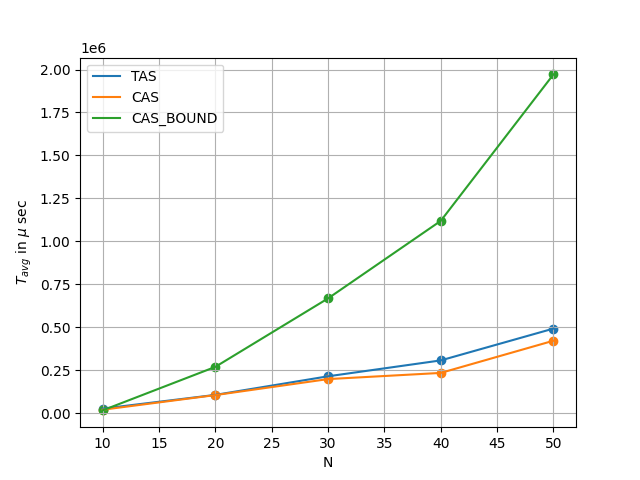
\includegraphics[width=0.79\textwidth]{average.png}
		\caption{$T_{avg}$ vs $N$ }
	\end{figure}
\pagebreak
	\subsubsection{Observations :}

		\begin{itemize}
			\item From the graph we can observe that using $TAS$ or $CAS$ we get nearly the same entering average time into CS.
			\item Average entering time is highest in case of $Bounded-CAS$.
		\end{itemize}

	\subsection{ Graph 2 :}
	\begin{itemize}
		\item The value of $K$ used by the program is fixed and is equal to $10$.
		\item Now we see the variation of max time of entering into CS ($T$) by varying the number of threads ($N$).
	\end{itemize}
	\subsubsection{Graph :}
	\begin{figure}[H]
		\centering
		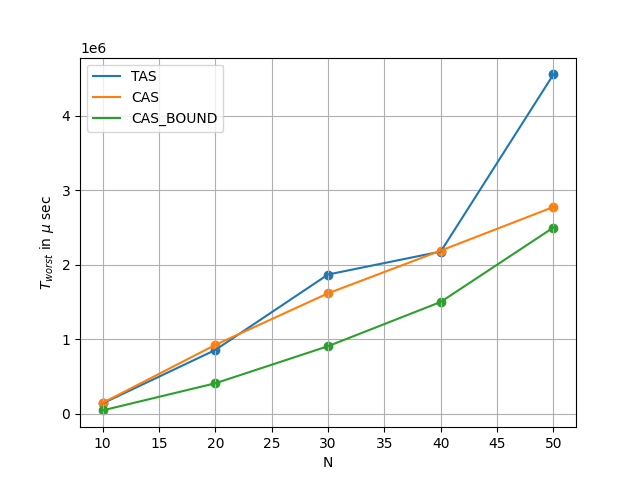
\includegraphics[width=0.8\textwidth]{worst.png}
		\caption{$T_{max}$ vs $N$ }
	\end{figure}
	\subsubsection{Observations :} 

		\begin{itemize}
	\item From the graph we can observe that using $TAS$ or $CAS$ we get nearly the same maximum entering time into CS for small values of $N$, but as value of $N$ increases for $TAS$ maximum entering time increases rapidly.
	\item Maximum entering time is lowest in case of $Bounded-CAS$.
\end{itemize}

	\section{ Final Conclusion:} 
	\begin{itemize}
		\item Maximum entering time is lowest in case of $Bounded-CAS$, and Average entering time is highest in case of $Bounded-CAS$.
	\end{itemize}
\end{document}



